\section{Reale Reaktoren}
Reale Reaktoren unterscheiden sich von idealen Reaktoren hinsichtlich:
\begin{itemize}
\item Radiale Konzentrations- oder Temperaturprofile
\item Axiale Dispersion (R�ckvermischung)
\item Ausbildung von Kan�len
\item Totr�ume
\item Kurzschluss-Str�me
\end{itemize}
Untersuchungen zum Str�mungsverhalten k�nnen selten am tats�chlichen Reaktor durchgef�hrt werden.
In den meisten F�llen wird hierf�r ein Modellreaktor im Laborma�stab herangezogen.
\subsection{Verweilzeitverteilung}
In realen Reaktoren entspricht die tats�chliche Verweilzeit (VWZ) nicht der hydrodynamischen VWZ $\tau=\frac{\dot V}{V}$, 
sondern folgt einer entsprechenden Altersverteilung.\\
VWZ-Verteilung am Reaktorausgang ({\sc exit}) durch Sto�markierung mit der definierten Menge $n_0$:
\[ \fbox{$\displaystyle E(t)=\frac{\dot n}{n_0}=\frac{\dot Vc(t)}{\int_0^{\infty}\dot Vc(t)dt}$} \]
\[ \int_0^{\infty}E(t)dt=1 \]
Das Integral der VWZ-Verteilung zwischen $t=0$ und $t=t_1$ entspricht dem Anteil an Molek�len, die k�rzer als $t_1$ im Reaktor verweilen.
\begin{figure}[H]
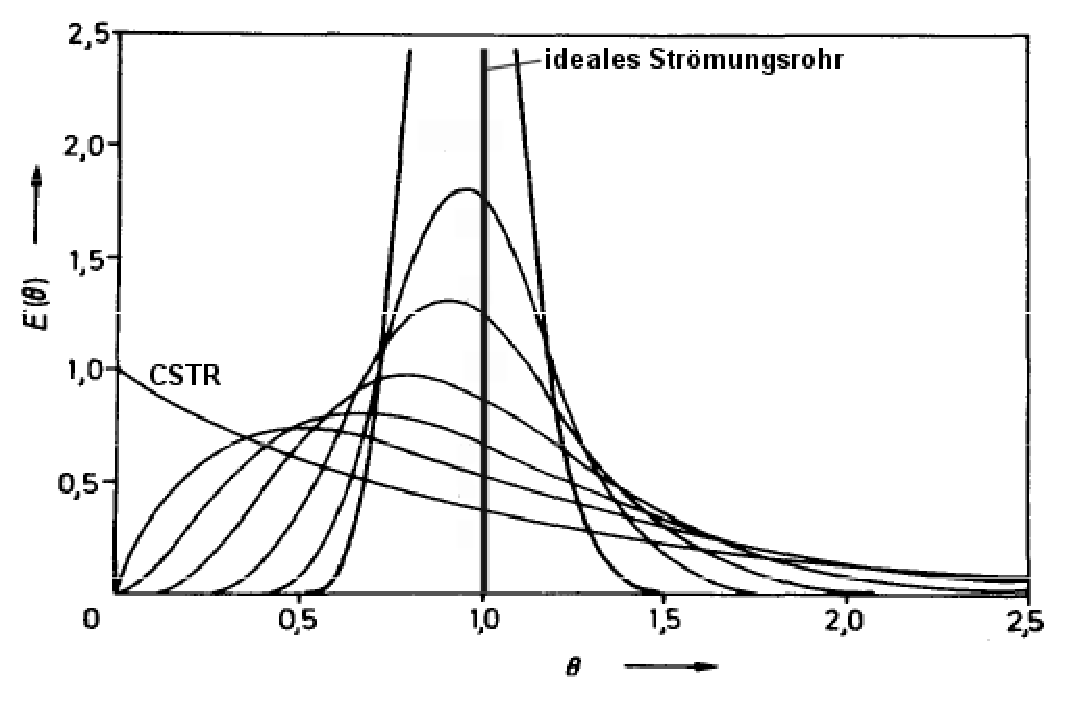
\includegraphics[width=87mm]{images/vwz-vert.eps}
\end{figure}
VWZ-Summenkurve (entspricht Verdr�ngungsmarkierung):
\[ \fbox{$\displaystyle F(t)=\int_0^tE(t)$} \]
\begin{figure}[H]
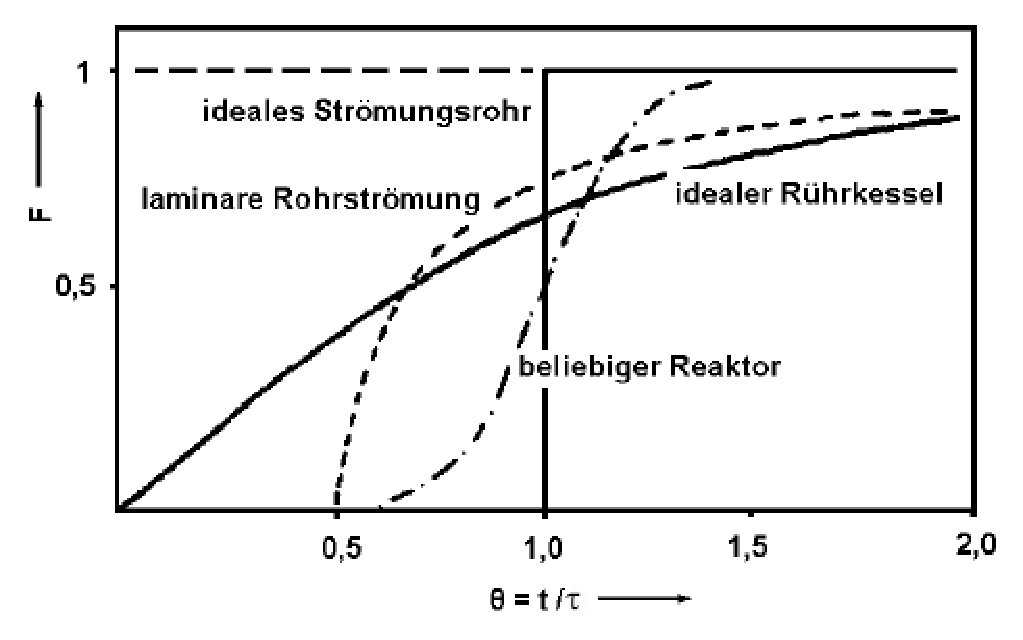
\includegraphics[width=87mm]{images/vwz-summe.eps}
\end{figure}
Interne VWZ-Verteilung:
\[ I(t)=\frac{1}{\tau}\left[1-F(t)\right] \]
F�r den idealen R�hrkessel (vollst�ndig r�ckvermischt) gilt: $I(t)=E(t)$\\
Die Zeitachse kann auch in der dimensionslosen Zeit
\[\fbox{$ \displaystyle \Theta=\frac{t}{\tau}$}\]
ausgedr�ckt werden.
\subsubsection{Beschreibung idealer Reaktoren}
Idealer PFTR:\\
\[ \fbox{$\displaystyle F(\Theta)=\left\{ \begin{array}{rcl}
   0 & : & 0<\Theta\leq1 \\
   1 & : & \Theta>1
 \end{array}
 \right.$} \]
Idealer STR:\\
\[ \fbox{$\displaystyle F(\Theta)=1-\exp{-\Theta}$} \]
\[ \fbox{$\displaystyle E(\Theta)=\frac{dF}{d\Theta}=\exp{-\Theta}$} \]

\subsection{Modelle realer Reaktoren}
\subsubsection{Dispersionsmodelle}
Dispersion ist ein {\it makroskopischer} Prozess, verursacht durch Varianzen des Str�mungsverhaltens (Turbulenz, etc.).\\
Massenbilanz mit Dispersionsterm f�r das eindimensionale Str�mungsrohr:\\
\[ \frac{\partial c}{\partial t}=-U\frac{\partial c}{\partial z}+D_z\frac{\partial^2c}{\partial z^2} \]
$D_z$ oder $D_{ax}$: Dispersionskoeffizient\\
{\sc Bodenstein}-Zahl:\\
\[ \fbox{$\displaystyle Bo=\frac{L\cdot U}{D_z}=\frac{\mbox{erzwungene Konvektion}}{\mbox{Dispersion}}$} \]
$Bo\rightarrow 0$: VWZ-Kurve n�hert sich dem idealen STR\\
$Bo\rightarrow \infty$: VWZ-Kurve n�hert sich dem PFTR\\
Axiale {\sc Peclet}-Zahl zur Bestimmung von $D_{ax}$ mittels empirischen Korrelationen:\\
\[ Pe_{ax}=\frac{\bar u d_R}{D_{ax}} \] 
\subsubsection{Kaskadenmodelle}
Das VWZ-Verhalten realer Reaktoren kann mit einer Reihenschaltung $N$ gleicher, ideal gemischter Zellen angen�hert werden.\\
\[ E(\Theta)=\frac{N\left(N\cdot \Theta\right)^{N-1}}{\left(N-1\right)!}\exp\left(-N\Theta\right) \]
Der Parameter $N$ wird durch Fitting der errechneten VWZ-Kurve mit der experimentell bestimmten VWZ-Kurve erhalten.\\
F�r $Bo>50$ gilt $Bo\approx2N$.
\subsubsection{Gemischte Modelle}
In manchen F�llen reichen die beiden Modelle mit jeweils nur einem Parameter nicht aus, um das beobachtete VWZ-Verhalten zu beschreiben.
In diesen F�llen werden gemischte Modelle (Kombination idealer Reaktoren) angewandt.
